\chapter{Convexity and Stability Analysis of the Single-hop Algorithm}
\label{chap:stability-singlehop}
In the previous chapter, we present DWARF, a physicomimetics desynchronization algorithm. From the evaluation results, the algorithm is eventually stable with low desynchronization error. 
However, it is not obvious that why DWARF is eventually stable with low error. 
Therefore, in this chapter, we mathematically analyse the stability of the algorithm.

We divide our analysis into two parts. First, we analyse the convexity of the force function. If the force function is convex, the system contains one global minima and no local minima. Therefore, the system could reach the perfect desynchrony state by gradually reducing the overall force of the system. Second, we analyse the stability when the system at the equilibrium. If the system is stable, it can be back to the equilibrium under a small perturbation. 

\section{Convexity Analysis}
\label{sec:convex}
In this section, our goal is to prove that the force function used in DWARF has one global minima and no local minima. In other words, we will prove that the force function is convex.

Let $F_{i}$ be the force summation at node $i$ and $\Delta_{i,j} \in (-\frac{T}{2}, \frac{T}{2})$  is an interval between node $i$ and $j$.
If $\Delta_{i,j} > 0$, the node $j$ repels the node $i$ in a positive direction.
In contrast,  if $\Delta_{i,j} < 0$, the node $j$ repels the node $i$ in a negative direction.

Therefore, for $n$ nodes, $F_{i}$ can be formulated as the following equation, 
\begin{equation}
F_{i} = \sum_{\substack{j=1\\j \neq i}}^{n} \frac{1}{\Delta_{i,j}}.
\end{equation}

The objective function $E$ of the system is the summation of absolute received forces at all nodes,
\begin{equation}
E = \sum_{i = 1}^{n}\left| F_{i} \right| = \sum_{i = 1}^{n} \left | \sum_{\substack{j=1\\j \neq i}}^{n} \frac{1}{\Delta_{i,j}} \right| 
\label{eq:energy}
\end{equation}
To prove the function $E$ is a convex function, we must prove that two following conditions are satisfied; 1) the set of all $\Delta_{i,j}$ is a convex set and 2) the Hessian matrix of $E$ is positive semidefinite. 

\begin{prop}
A set of all possible interval $\Delta_{i,j}$ is a convex set.
\label{prop:convexset}
\end{prop}
\begin{proof}
A set of $(-\frac{T}{2}, \frac{T}{2})$ is a line connecting between $-\frac{T}{2}$ and $\frac{T}{2}$. 
Therefore, any $\Delta_{i_1,j_1}$, $\Delta_{i_2,j_2} \in$  $(-\frac{T}{2}, \frac{T}{2})$ and $\alpha \in \mathbb{R}$ with $0 \le \alpha \le 1$,
\begin{equation}
\alpha\Delta_{i_1,j_1} + (1-\alpha)\Delta_{i_2,j_2} \in (-\frac{T}{2}, \frac{T}{2}). \nonumber
\end{equation} 
\end{proof}

\begin{prop}
The Hessian of the function $E$ is positive semidefinite.
\label{prop:Hessian}
\end{prop}

\begin{proof}
Let $H$ be the Hessian matrix of the objective function $E$,

$H = 
\begin{pmatrix} 
{\frac{\partial^2 E}{\partial \Delta_{1,2}^2}}  & {\frac{\partial^2 E}{\partial \Delta_{1,2}\partial\Delta_{1,3}}}  & \cdots & {\frac{\partial^2 E}{\partial \Delta_{1,2}\partial \Delta_{n,n-1}}} \\ 
{\frac{\partial^2 E}{\partial \Delta_{1,3}\partial \Delta_{1,2}}}  & {\frac{\partial^2 E}{\partial \Delta_{1,3}^2}} & \cdots & {\frac{\partial^2 E}{\partial \Delta_{1,3}\partial \Delta_{n,n-1}}} \\ 
\vdots & \vdots & \ddots & \vdots \\
{\frac{\partial^2 E}{\partial \Delta_{n,n-1}\partial \Delta_{1,2}}} & {\frac{\partial^2 E}{\partial \Delta_{n,n-1}\partial \Delta_{1,3}}} & \cdots & {\frac{\partial^2 E}{\partial \Delta_{n,n-1}^2}}
\end{pmatrix}$.

For any $\Delta_{x,y}$, we derive the first-order derivative as follows,
\begin{equation}
{\frac{\partial E}{\partial \Delta_{x,y}}} = \frac{\sum_{\substack{j=1\\j \neq x}}^{n} \frac{1}{\Delta_{x,j}} }{\left| \sum_{\substack{j=1\\j \neq x}}^{n} \frac{1}{\Delta_{x,j}} \right|} \left( - \frac{1}{\Delta_{x,y}^2} \right). \nonumber
\end{equation}

For the second-order partial derivatives, if we differentiate with the same $\Delta_{x,y}$, 
\begin{alignat}{2}
{\frac{\partial^2 E}{\partial \Delta_{x,y}^2}} = \frac{\sum_{\substack{j=1\\j \neq x}}^{n} \frac{1}{\Delta_{x,j}} }{\left| \sum_{\substack{j=1\\j \neq x}}^{n} \frac{1}{\Delta_{x,j}} \right|} \left( \frac{2}{\Delta_{x,y}^3} \right). \nonumber
\end{alignat}

In the other hand, if we differentiate with other $\Delta_{u,v}$, where $u \neq x$ or $v \neq y$, ${\frac{\partial^2}{\partial \Delta_{u,v}\partial\Delta_{x,y}}}E = 0$.

Therefore, the Hessian matrix of the function $E$ is

$H = 
\begin{pmatrix} 
a_{1,2} & 0 & \cdots & 0 \\ 
0 & a_{1,3} & \cdots & 0 \\ 
\vdots & \vdots & \ddots & \vdots \\
0 & 0 & \cdots & a_{n, n-1} \\ 
\end{pmatrix}$,

where $a_{i,j} = \frac{u_{i}}{|u_{i}|} \left( \frac{2}{\Delta_{i,j}^3} \right)$ and $u_{i} = \sum_{\substack{j=1\\j \neq i}}^{n}  \frac{1}{\Delta_{i,j}}$.

To show that the Hessian matrix of the function $E$ is positive semidefinite, we show that $\vec{\Delta}^{T}H\vec{\Delta} \geq 0$ for all $\vec{\Delta}$ when $\vec{\Delta} \neq 0$.

\begin{alignat}{2}
\vec{\Delta}^{T}H\vec{\Delta} &=
\begin{pmatrix}
 \Delta_{1,2} & \Delta_{1,3} & \cdots & \Delta_{n,n-1} \\
\end{pmatrix}
H
\begin{pmatrix}
 \Delta_{1,2} \\
 \Delta_{1,3} \\
 \vdots \\
 \Delta_{n,n-1}
\end{pmatrix} \nonumber \\
=& \text{ } \sum_{i = 1}^{n} \sum_{\substack{j=1\\j \neq i}}^{n} \frac{u_{i}}{|u_{i}|}  \left( \frac{2}{\Delta_{i,j}} \right) \nonumber \\
=& \text{ } 2 \sum_{i = 1}^{n} \frac{u_{i}}{|u_{i}|} \sum_{\substack{j=1\\j \neq i}}^{n}  \frac{1}{\Delta_{i,j}} \nonumber \\
=& \text{ } 2 \sum_{i = 1}^{n} \frac{u_{i}}{|u_{i}|} u_{i} = 2 \sum_{i = 1}^{n} |u_{i}| \nonumber \\
\geq& \text{ } 0 \nonumber
\end{alignat}

Therefore, we conclude that $\vec{\Delta}^{T}H\vec{\Delta} \geq 0$ and the Hessian matrix of $E$ is positive semidefinite.  
\end{proof}

From Proposition \ref{prop:convexset} and \ref{prop:Hessian}, we derive the following lemma.
\begin{lem}
the function $E$ is a convex function.
\label{lemma:convexset}
\end{lem}

From the above lemma, we finish our proof with the following theorem.

\begin{thm}
The system force summation function of DWARF has one global minima and no local minima.
\label{theorem:minima}
\end{thm}

\section{Stability Analysis}
\label{sec:stability}
To prove that the system is stable, we begin by transforming the system into a non-linear dynamic system. 
The evenness of the number of nodes affects the analysis. Therefore, we divide the non-linear dynamic system into two cases: when $n$ is even and when $n$ is odd where $n$ is the number of nodes.

1) when $n$ is even: Figure \ref{fig:even-perfect} illustrates the equilibrium of a dynamic system when the number of nodes is even. Noticeably, node 0 and $n/2$ are exactly at the opposite side of each other. At the first snapshot of the system, node 0 adjusts its phase based on the force function of DWARF. After adjustment, we re-label node 1 to 0, node 2 to 1, ..., node $n-1$ to $n-2$, and node 0 to $n-1$ for analysis at the next snapshot (see Figure \ref{fig:even-adapt}).
Therefore, to transform into a difference equation, $\Delta_{1}$ in the next snapshot is $\Delta_{2}$ in the previous snapshot, $\Delta_{2}$ in the next snapshot is $\Delta_{3}$ in the previous snapshot, and so on. However, $\Delta_{n-1}$ and $\Delta_{n}$ in the next snapshot are $\Delta_{n}$ and $\Delta_{1}$ in the previous snapshot adjusted by the force function, respectively.
\begin{figure*}[!t]
\centerline{
	\subfloat[]{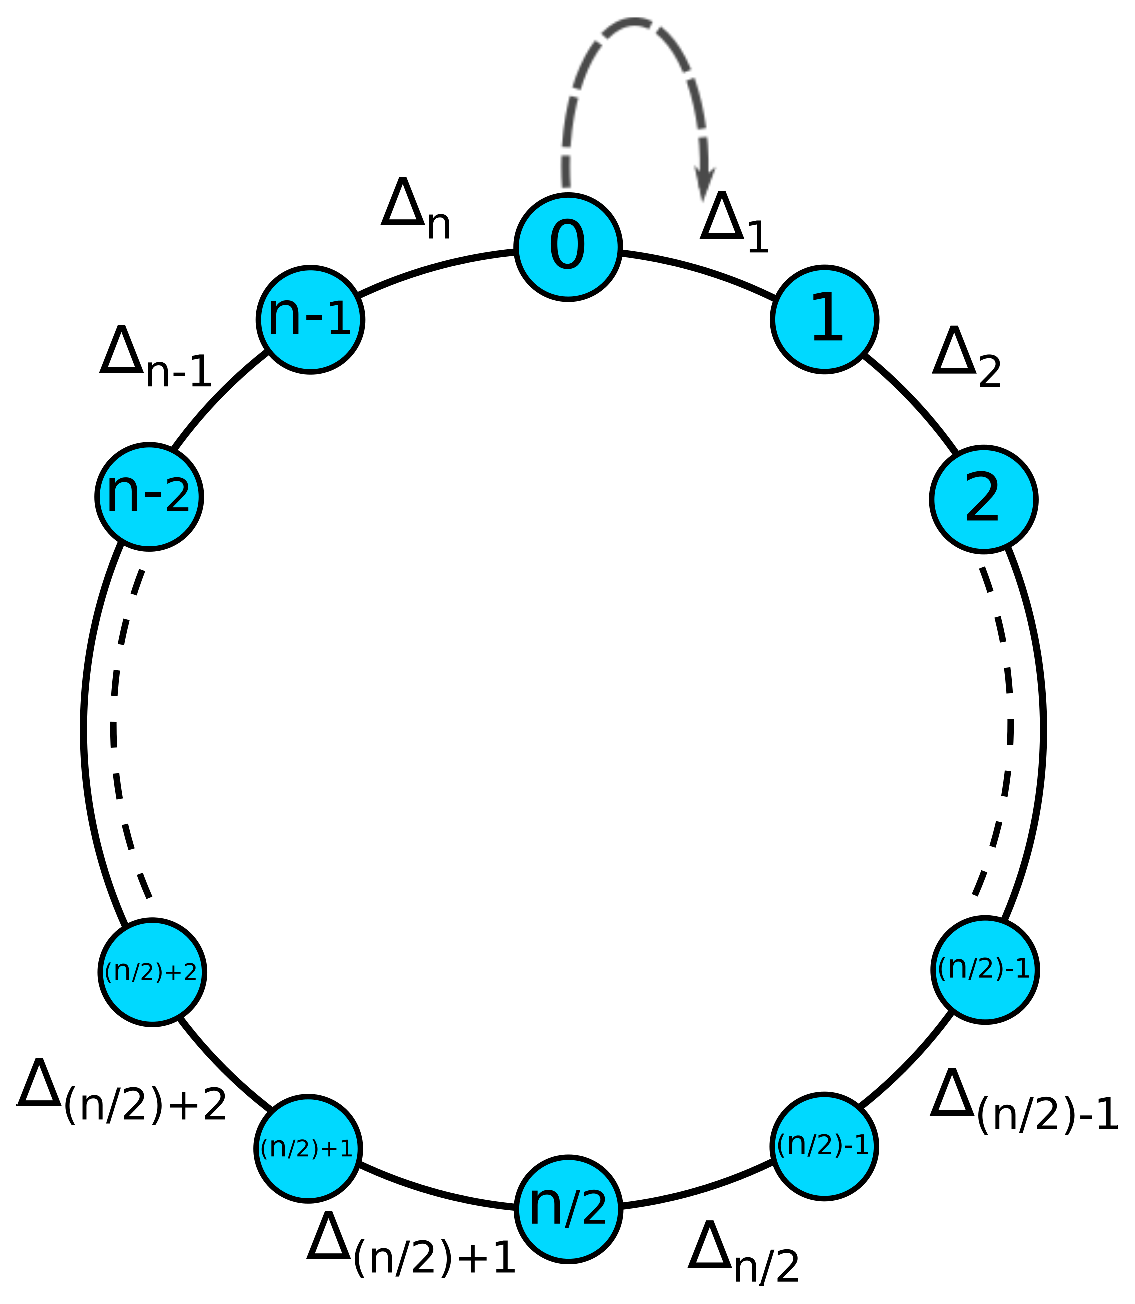
\includegraphics[scale=0.30]{figure/stability-onehop-even}%
	\label{fig:even-perfect}}
	\hfil
	\subfloat[]{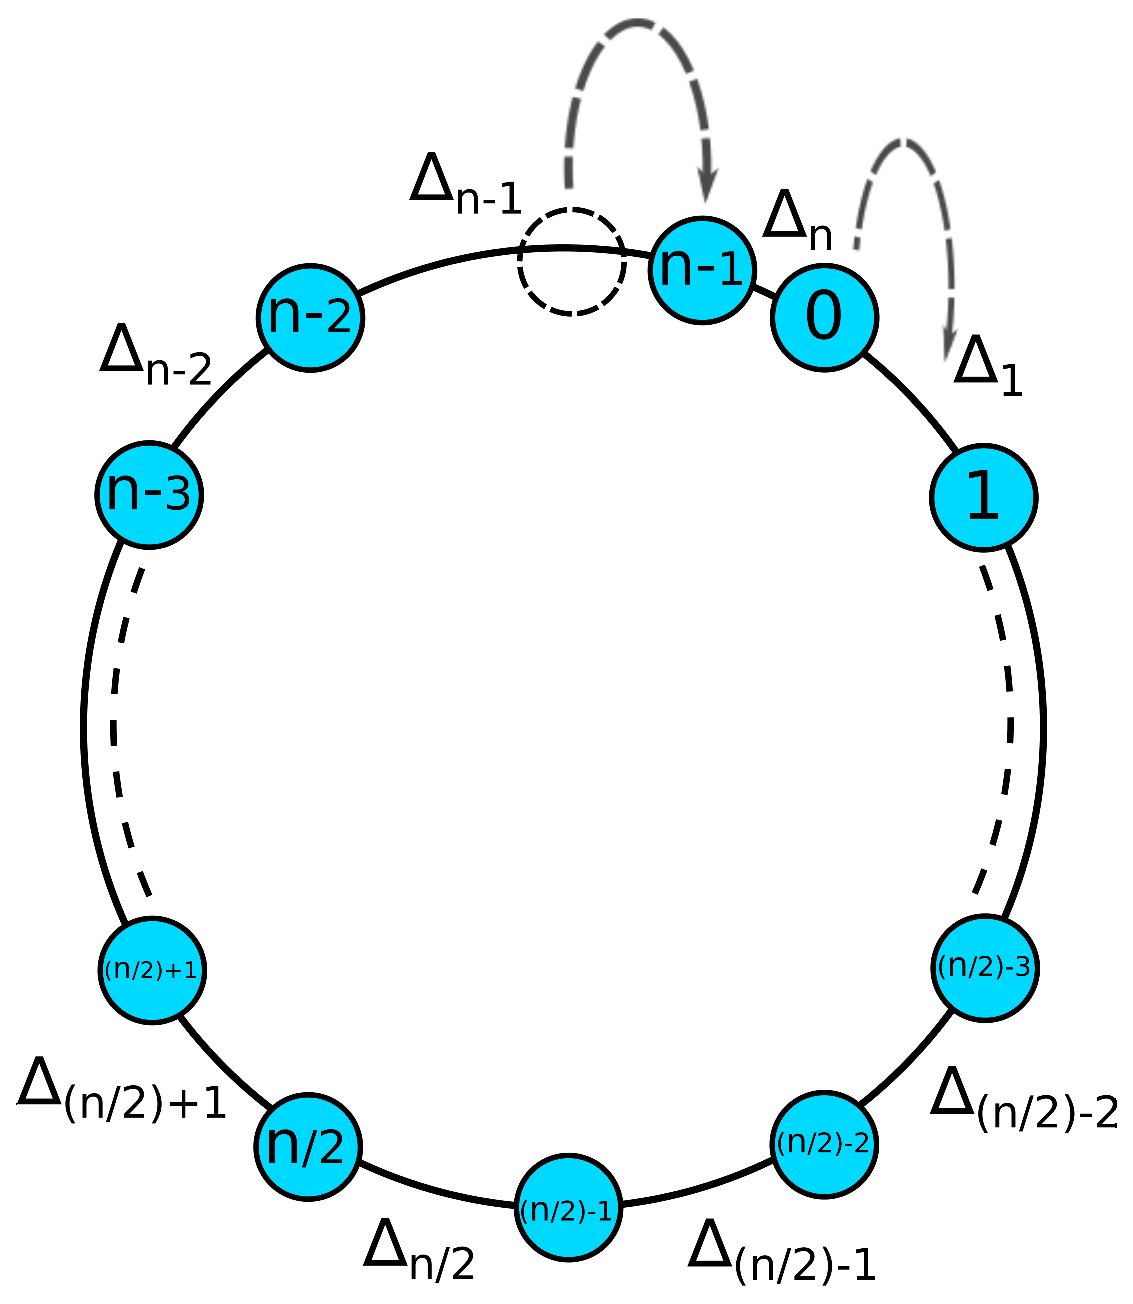
\includegraphics[scale=0.30]{figure/stability-onehop-even-adapt}%
	\label{fig:even-adapt}}
}
\caption{Non-linear dynamic system when $n$ is even. (a) The snapshot of the system at one time step. (b) In next time step after node 0 adjusts its phase, node 1 in previous round is re-labelled to 0, node 2 is re-labelled to 1, and so on.}
\label{fig:n-even}
\lofcont
\end{figure*}
Therefore, the non-linear dynamic system when $n$ is even can be expressed as the following difference equations:

\begin{alignat}{1}
 \Delta_{1} =& \Delta_{2} \nonumber \\
 \Delta_{2} =& \Delta_{3} \nonumber \\
 \vdots \nonumber \\
 \Delta_{n-2} =& \Delta_{n-1} \nonumber \\
 \Delta_{n-1} =& \Delta_{n} + KT\Bigg( -\frac{1}{\Delta_{1}} - \frac{1}{\Delta_{1} + \Delta_{2}} - \hdots - \frac{1}{\Delta_{1} + \Delta_{2} + \hdots + \Delta_{\frac{n}{2}-1}} \nonumber \\ 
&+ \frac{1}{\Delta_{n}} + \frac{1}{\Delta_{n} + \Delta_{n-1}} + \hdots + \frac{1}{\Delta_{n} + \Delta_{n-1} + \hdots + \Delta_{\frac{n}{2}+2}}\Bigg) \nonumber \\
 \Delta_{n} =& \Delta_{1} - KT\Bigg( -\frac{1}{\Delta_{1}} - \frac{1}{\Delta_{1} + \Delta_{2}} - \hdots - \frac{1}{\Delta_{1} + \Delta_{2} + \hdots + \Delta_{\frac{n}{2}-1}} \nonumber \\ 
&+ \frac{1}{\Delta_{n}} + \frac{1}{\Delta_{n} + \Delta_{n-1}} + \hdots + \frac{1}{\Delta_{n} + \Delta_{n-1} + \hdots + \Delta_{\frac{n}{2}+2}}\Bigg) 
\end{alignat}

We note that the force from node $n/2$ in the previous snapshot is already balanced when we consider node 0. Therefore, $\Delta_{\frac{n}{2}}$ and $\Delta_{\frac{n}{2}+1}$ do not appear in the force equation for adjusting $\Delta_{n-1}$ and $\Delta_{n}$ in the next snapshot.

2) when $n$ is odd:
Similarly, Figure \ref{fig:n-odd} illustrates the non-linear dynamic system when $n$ is odd. The only difference from when $n$ is even is that there is no node that is opposite to node 0. Therefore, in the difference equations, only $\Delta_{\lceil\frac{n}{2}\rceil}$ from the previous snapshot does not appear in the force equation for adjusting $\Delta_{n-1}$ and $\Delta_{n}$ in the next snapshot.
\begin{figure*}[!t]
\centerline{
	\subfloat[]{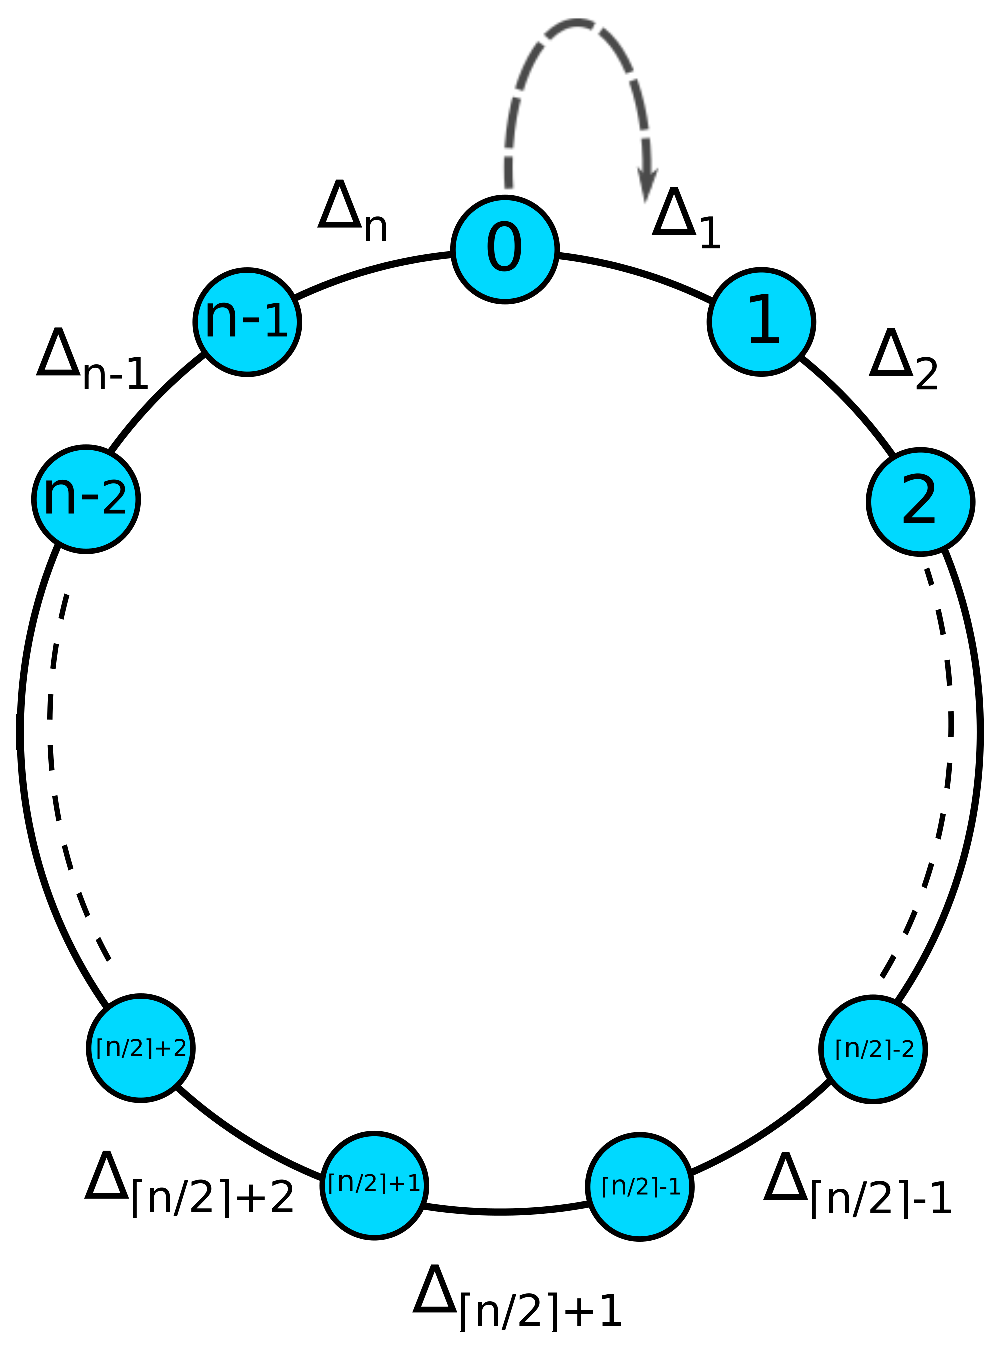
\includegraphics[scale=0.30]{figure/stability-onehop-odd}%
	\label{fig:odd}}
	\hfil
	\subfloat[]{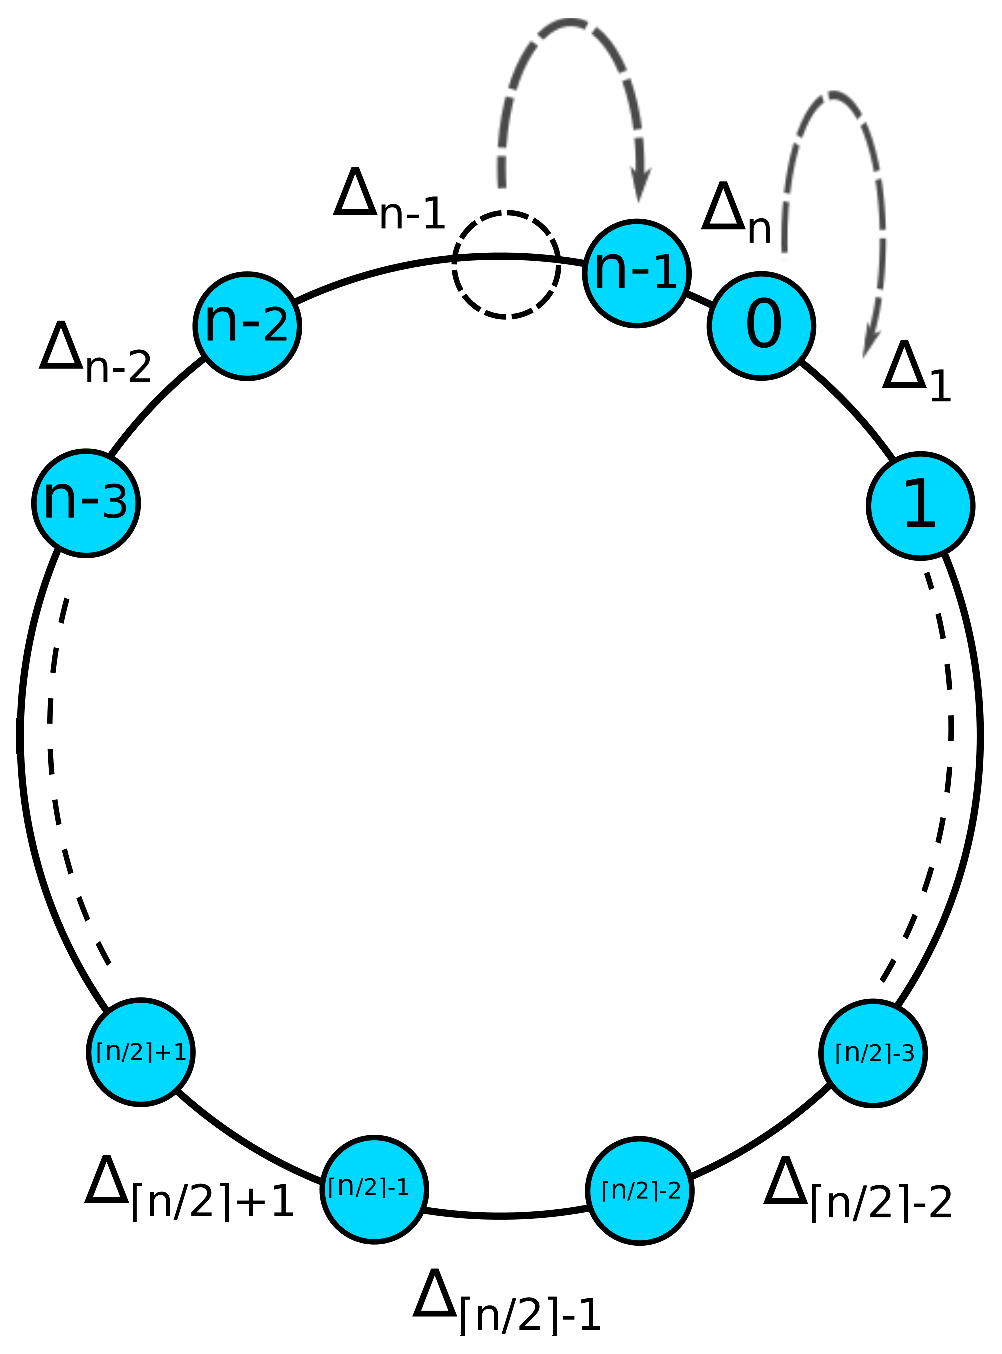
\includegraphics[scale=0.30]{figure/stability-onehop-odd-adapt}%
	\label{fig:odd-adapt}}
}
\caption{Non-linear dynamic system when $n$ is odd. (a) The snapshot of the system at one time step. (b) In next time step after node 0 adjusts its phase, node 1 in previous round is re-labelled to 0, node 2 is re-labelled to 1, and so on.}
\label{fig:n-odd}
\lofcont
\end{figure*}
\begin{alignat}{1}
 \Delta_{1} =& \Delta_{2} \nonumber \\
 \Delta_{2} =& \Delta_{3} \nonumber \\
 \vdots \nonumber \\
 \Delta_{n-2} =& \Delta_{n-1} \nonumber \\
 \Delta_{n-1} =& \Delta_{n} + KT\Bigg( -\frac{1}{\Delta_{1}} - \frac{1}{\Delta_{1} + \Delta_{2}} - \hdots - \frac{1}{\Delta_{1} + \Delta_{2} + \hdots + \Delta_{\lceil{\frac{n}{2}}\rceil-1}} \nonumber \\ 
&+ \frac{1}{\Delta_{n}} + \frac{1}{\Delta_{n} + \Delta_{n-1}} + \hdots + \frac{1}{\Delta_{n} + \Delta_{n-1} + \hdots + \Delta_{\lceil\frac{n}{2}\rceil+1}}\Bigg) \nonumber \\
 \Delta_{n} =& \Delta_{1} - KT\Bigg( -\frac{1}{\Delta_{1}} - \frac{1}{\Delta_{1} + \Delta_{2}} - \hdots - \frac{1}{\Delta_{1} + \Delta_{2} + \hdots + \Delta_{\lceil\frac{n}{2}\rceil-1}} \nonumber \\ 
&+ \frac{1}{\Delta_{n}} + \frac{1}{\Delta_{n} + \Delta_{n-1}} + \hdots + \frac{1}{\Delta_{n} + \Delta_{n-1} + \hdots + \Delta_{\lceil\frac{n}{2}\rceil+1}}\Bigg) \nonumber 
\end{alignat}

Due to the non-linear adaptation function, the standard linear dynamic system analysis does not suffice.
Therefore, we locally analyse stability of the system around a fixed point which is the equilibrium point.
We begin by linear approximation to find the Jacobian at the equilibrium. Then, from the Jacobian, we find the bound of eigenvalues which is the crucial part of stability analysis.


\subsection{Linear Approximation}
The Jacobian ($J$) of a difference equations system is defined as follows:

\begin{alignat}{2}
J=\begin{pmatrix} 
{\frac{\partial \Delta_{1}}{\partial \Delta_{1}}}  & {\frac{\partial \Delta_{1}}{\partial \Delta_{2}}} & \cdots & {\frac{\partial \Delta_{1}}{\partial \Delta_{n-1}}} & {\frac{\partial \Delta_{1}}{\partial \Delta_{n}}} \\ 
{\frac{\partial \Delta_{2}}{\partial \Delta_{1}}}  & {\frac{\partial \Delta_{2}}{\partial \Delta_{2}}} & \cdots &  {\frac{\partial \Delta_{2}}{\partial \Delta_{n-1}}} & {\frac{\partial \Delta_{2}}{\partial \Delta_{n}}} \\  
\vdots & \vdots & \ddots & \vdots & \vdots \\
{\frac{\partial \Delta_{n-1}}{\partial \Delta_{1}}} & {\frac{\partial \Delta_{n-1}}{\partial \Delta_{2}}} & \cdots &  {\frac{\partial \Delta_{n-1}}{\partial \Delta_{n-1}}} & {\frac{\partial \Delta_{n-1}}{\partial \Delta_{n}}} \\  
{\frac{\partial \Delta_{n}}{\partial \Delta_{1}}} & {\frac{\partial \Delta_{n}}{\partial \Delta_{2}}} & \cdots &  {\frac{\partial \Delta_{n}}{\partial \Delta_{n-1}}} & {\frac{\partial \Delta_{n}}{\partial \Delta_{n}}} \\  
\end{pmatrix}
\end{alignat}

We consider the Jacobian when $n$ is even and odd separately. In both cases, after finding the Jacobian, we substitute each $\Delta_{i}$ with $T/n$ which is the phase interval between each node at the equilibrium.

1) $n$ is even:

For $\Delta_{i}, 1 \leq i \leq n-2$, partial derivatives of ${\partial \Delta_{i} / \partial \Delta_{j}}, 1 \leq j \leq n$ are the followings:
\begin{alignat}{1}
  {\frac{\partial \Delta_{i}}{\partial \Delta_{j}}} = \left\{ 
  \begin{array}{l l}
    1 & \quad \text{if } j = i + 1\\
    0 & \quad \text{otherwise}\\
  \end{array} \right. \nonumber
\end{alignat}


For $\Delta_{n-1}$, we find its partial derivatives as follows:
\begin{alignat}{1}
{\frac{\partial \Delta_{n-1}}{\partial \Delta_{1}}} =& KT\left(\frac{1}{\Delta_1^2} + \frac{1}{(\Delta_1 + \Delta_2)^2} + \cdots + \frac{1}{(\Delta_1 + \Delta_2 + \cdots + \Delta_{\frac{n}{2}-1})^2}\right) \nonumber \\
=&KT\left(\frac{n^2}{T^2}\right)\left(\frac{1}{1^2} + \frac{1}{2^2} + \cdots + \frac{1}{(\frac{n}{2}-1)^2}\right) = \frac{Kn^2}{T} \sum\limits_{i=1}^{\frac{n}{2}-1}{\frac{1}{i^2}} \nonumber \\
{\frac{\partial \Delta_{n-1}}{\partial \Delta_{2}}} =& KT\left(\frac{1}{(\Delta_1 + \Delta_2)^2} + \cdots + \frac{1}{(\Delta_1 + \Delta_2 + \cdots + \Delta_{\frac{n}{2}-1})^2}\right) \nonumber \\
=&KT\left(\frac{n^2}{T^2}\right)\left(\frac{1}{2^2} + \cdots + \frac{1}{(\frac{n}{2}-1)^2}\right) = \frac{Kn^2}{T} \sum\limits_{i=2}^{\frac{n}{2}-1}{\frac{1}{i^2}} \nonumber \\
\vdots \nonumber \\
{\frac{\partial \Delta_{n-1}}{\partial \Delta_{\frac{n}{2}-1}}} =& KT\left(\frac{1}{(\Delta_1 + \Delta_2 + \cdots + \Delta_{\frac{n}{2}-1})^2}\right) \nonumber \\
=&KT\left(\frac{n^2}{T^2}\right)\left(\frac{1}{(\frac{n}{2}-1)^2}\right) = \frac{Kn^2}{T} \sum\limits_{i=\frac{n}{2}-1}^{\frac{n}{2}-1}{\frac{1}{i^2}} \nonumber \\	
{\frac{\partial \Delta_{n-1}}{\partial \Delta_{\frac{n}{2}}}} =& 0 \nonumber \\
{\frac{\partial \Delta_{n-1}}{\partial \Delta_{\frac{n}{2}+1}}} =& 0 \nonumber \\
{\frac{\partial \Delta_{n-1}}{\partial \Delta_{\frac{n}{2}+2}}} =& KT\left(-\frac{1}{(\Delta_n + \Delta_{n-1} + \cdots + \Delta_{\frac{n}{2}+2})^2}\right) \nonumber \\
=&-KT\left(\frac{n^2}{T^2}\right)\left(\frac{1}{(\frac{n}{2}-1)^2}\right) = -\frac{Kn^2}{T} \sum\limits_{i=\frac{n}{2}-1}^{\frac{n}{2}-1}{\frac{1}{i^2}} \nonumber \\	
\vdots \nonumber \\
{\frac{\partial \Delta_{n-1}}{\partial \Delta_{n-1}}} =& KT\left(-\frac{1}{(\Delta_n + \Delta_{n-1})^2} - \cdots - \frac{1}{(\Delta_n + \Delta_{n-1} + \cdots + \Delta_{\frac{n}{2}+2})^2}\right) \nonumber \\
=&-KT\left(\frac{n^2}{T^2}\right)\left(\frac{1}{2^2} + \cdots + \frac{1}{(\frac{n}{2}-1)^2}\right) = -\frac{Kn^2}{T} \sum\limits_{i=2}^{\frac{n}{2}-1}{\frac{1}{i^2}} \nonumber \\
{\frac{\partial \Delta_{n-1}}{\partial \Delta_{n}}} =& 1+KT\left(-\frac{1}{\Delta_n^2} - \frac{1}{(\Delta_n + \Delta_{n-1})^2} - \cdots - \frac{1}{(\Delta_n + \Delta_{n-1} + \cdots + \Delta_{\frac{n}{2}+2})^2}\right) \nonumber  \\
=&1-KT\left(\frac{n^2}{T^2}\right)\left(\frac{1}{1^2} + \frac{1}{2^2} + \cdots + \frac{1}{(\frac{n}{2}-1)^2}\right) = 1-\frac{Kn^2}{T} \sum\limits_{i=1}^{\frac{n}{2}-1}{\frac{1}{i^2}} \nonumber 
\end{alignat}

For $\Delta_{n}$, we find its partial derivatives which is similar to $\Delta_{n-1}$ as follows.

\begin{alignat}{1}
{\frac{\partial \Delta_{n}}{\partial \Delta_{1}}} =& 1-\frac{Kn^2}{T} \sum\limits_{i=1}^{\frac{n}{2}-1}{\frac{1}{i^2}} \nonumber \\
{\frac{\partial \Delta_{n}}{\partial \Delta_{2}}} =& -\frac{Kn^2}{T} \sum\limits_{i=2}^{\frac{n}{2}-1}{\frac{1}{i^2}} \nonumber \\
\vdots \nonumber \\
{\frac{\partial \Delta_{n}}{\partial \Delta_{\frac{n}{2}-1}}} =& -\frac{Kn^2}{T} \sum\limits_{i=\frac{n}{2}-1}^{\frac{n}{2}-1}{\frac{1}{i^2}} \nonumber \\	
{\frac{\partial \Delta_{n}}{\partial \Delta_{\frac{n}{2}}}} =& 0 \nonumber \\
{\frac{\partial \Delta_{n}}{\partial \Delta_{\frac{n}{2}+1}}} =& 0 \nonumber \\
{\frac{\partial \Delta_{n}}{\partial \Delta_{\frac{n}{2}+2}}} =& \frac{Kn^2}{T} \sum\limits_{i=\frac{n}{2}-1}^{\frac{n}{2}-1}{\frac{1}{i^2}} \nonumber \\	
\vdots \nonumber \\
{\frac{\partial \Delta_{n}}{\partial \Delta_{n-1}}} =& \frac{Kn^2}{T} \sum\limits_{i=2}^{\frac{n}{2}-1}{\frac{1}{i^2}} \nonumber \\
{\frac{\partial \Delta_{n}}{\partial \Delta_{n}}} =& \frac{Kn^2}{T} \sum\limits_{i=1}^{\frac{n}{2}-1}{\frac{1}{i^2}} \nonumber 
\end{alignat}

Let $\sum\limits_{s}$ stands for $\sum\limits_{i=s}^{\frac{n}{2}-1}{\frac{1}{i^2}}$, where $s \in [1,\frac{n}{2}-1]$ and let $A = Kn^2/T$.
The Jacobian matrix of the system, when $n$ is even, is

\begin{alignat}{1}
J=\begin{pmatrix}
 0 & 1  & \cdots & 0 & 0 & 0 & 0 & \cdots & 0 & 0\\ 
 0 & 0  & \ddots & 0 & 0 & 0 & 0 & \cdots & 0 & 0\\  
\vdots & \vdots & \ddots & \ddots & \vdots & \vdots & \vdots & \ddots & \vdots & \vdots\\
 0 & 0  & \cdots & 0 & 1 & 0 & 0 & \cdots & 0 & 0\\  
 0 & 0  & \cdots & 0 & 0 & 1 & 0 & \cdots & 0 & 0\\  
 0 & 0 & \cdots & 0 & 0 & 0 & 1 & \cdots & 0 & 0\\  
\vdots & \vdots & \ddots & \vdots & \vdots & \vdots & \vdots & \ddots & \vdots & \vdots\\
 0 & 0  & \cdots & 0 & 0 & 0 & 0 & \cdots & 1 & 0 \\ 
A\sum\limits_{1} & A\sum\limits_{2} & \cdots &  A\sum\limits_{\frac{n}{2}-1} & 0 & 0 & - A\sum\limits_{\frac{n}{2}-1}& \cdots & - A\sum\limits_{2} & 1 - A\sum\limits_{1} \\  
1 - A\sum\limits_{1} & - A\sum\limits_{2} & \cdots &  - A\sum\limits_{\frac{n}{2}-1} & 0 & 0 &  A\sum\limits_{\frac{n}{2}-1}& \cdots & A\sum\limits_{2} & A\sum\limits_{1} \\  
\end{pmatrix}.
\end{alignat}

2) $n$ is odd:

Similarly, when $n$ is odd, we can find its Jacobian with the same procedure as when $n$ is even.
We obtain the similar Jacobian matrix as follows: 

\begin{alignat}{1}
J=\begin{pmatrix}
 0 & 1  & \cdots & 0 & 0 & 0 & \cdots & 0 & 0\\ 
 0 & 0  & \ddots & 0 & 0 & 0 & \cdots & 0 & 0\\  
\vdots & \vdots & \ddots & \ddots & \vdots & \vdots & \ddots & \vdots & \vdots\\
 0 & 0  & \cdots & 0 & 1  & 0 & \cdots & 0 & 0\\  
 0 & 0  & \cdots & 0 & 0 & 1 & \cdots & 0 & 0\\  
\vdots & \vdots & \ddots & \vdots & \vdots & \vdots & \ddots & \vdots & \vdots\\
 0 & 0  & \cdots & 0 & 0 & 0 & \cdots & 1 & 0 \\ 
A\sum\limits_{1} & A\sum\limits_{2} & \cdots &  A\sum\limits_{\frac{n}{2}-1} & 0 & - A\sum\limits_{\frac{n}{2}-1}& \cdots & - A\sum\limits_{2} & 1 - A\sum\limits_{1} \\  
1 - A\sum\limits_{1} & - A\sum\limits_{2} & \cdots &  - A\sum\limits_{\frac{n}{2}-1} & 0 &  A\sum\limits_{\frac{n}{2}-1}& \cdots & A\sum\limits_{2} & A\sum\limits_{1} \\  
\end{pmatrix}.
\end{alignat}


\subsection{Finding Eigenvalues}
After finding the Jacobian of the linear approximation at the equilibrium, we find the eigenvalues by solving the equation $|J-\lambda I| = 0$. If all eigenvalues lay on a unit circle, the system is stable at the equilibrium. Therefore, we begin by finding the determinant of the matrix $J-\lambda I$. 
We use row operations to transform the determinant of $|J-\lambda I|$ into the determinant of a triangular matrix. Then, the determinant of the triangular matrix is the multiplication of diagonal entries. 

The following procedure is to transform the determinant of $|J-\lambda I|$ into the determinant of triangular matrix when $n$ is even:

\begingroup
\small
\begin{alignat}{1}
|J-\lambda I| &=\begin{vmatrix} 
-\lambda  & 1 & \cdots & 0 & 0 & 0 & 0 & \cdots & 0 & 0\\ 
0  & -\lambda  & \ddots & 0 & 0 & 0 & 0 & \cdots & 0 & 0\\  
\vdots & \vdots & \ddots & \ddots & \vdots & \vdots & \vdots & \ddots & \vdots & \vdots\\
0  & 0  & \cdots & -\lambda & 1 & 0 & 0 & \cdots & 0 & 0\\  
0  & 0  & \cdots & 0 & -\lambda & 1 & 0 & \cdots & 0 & 0\\  
0  & 0  & \cdots & 0 & 0 & -\lambda & 1 & \cdots & 0 & 0\\  
\vdots & \vdots & \ddots & \vdots & \vdots & \vdots & \ddots & \ddots & \vdots & \vdots\\
0  & 0  & \cdots & 0 & 0 & 0 & 0 & \cdots & 1 & 0 \\ 
A\sum\limits_{1} & A\sum\limits_{2} & \cdots &  A\sum\limits_{\frac{n}{2}-1} & 0 & 0 & -A\sum\limits_{\frac{n}{2}-1}& \cdots & -A\sum\limits_{2}-\lambda & 1-A\sum\limits_{1} \\  
1-A\sum\limits_{1} & -A\sum\limits_{2} & \cdots &  -A\sum\limits_{\frac{n}{2}-1} & 0 & 0 &  A\sum\limits_{\frac{n}{2}-1}& \cdots & A\sum\limits_{2} & A\sum\limits_{1}-\lambda \\  
\end{vmatrix} \\
&=\begin{vmatrix} 
-\lambda  & 1  & \cdots & 0 & 0 & 0 & 0 & \cdots & 0 & 0\\ 
0  & -\lambda  & \ddots & 0 & 0 & 0 & 0 & \cdots & 0 & 0\\  
\vdots & \vdots & \ddots & \ddots & \vdots & \vdots & \vdots & \ddots & \vdots & \vdots\\
0  & 0  & \cdots & -\lambda & 1 & 0 & 0 & \cdots & 0 & 0\\  
0  & 0  & \cdots & 0 & -\lambda & 1 & 0 & \cdots & 0 & 0\\  
0  & 0  & \cdots & 0 & 0 & -\lambda & 1 & \cdots & 0 & 0\\  
\vdots & \vdots & \ddots & \vdots & \vdots & \vdots & \ddots & \ddots & \vdots & \vdots\\
0  & 0  & \cdots & 0 & 0 & 0 & 0 & \cdots & 1 & 0 \\ 
1 & 0 & \cdots &  0 & 0 & 0 & 0 & \cdots & -\lambda & 1-\lambda \\  
1-A\sum\limits_{1} & -A\sum\limits_{2} & \cdots &  -A\sum\limits_{\frac{n}{2}-1} & 0 & 0 &  A\sum\limits_{\frac{n}{2}-1}& \cdots & A\sum\limits_{2} & A\sum\limits_{1}-\lambda \\  
\end{vmatrix} \\
&=\begin{vmatrix} 
-\lambda + \frac{1}{\lambda^{n-2}}  & 0  & \cdots & 0 & 0 & 0 & 0 & \cdots & 0 &  \frac{1-\lambda}{\lambda^{n-2}}\\ 
\frac{1}{\lambda^{n-3}}  & -\lambda  & \cdots & 0 & 0 & 0 & 0 & \cdots & 0 &  \frac{1-\lambda}{\lambda^{n-3}} \\ 
\frac{1}{\lambda^{n-4}}  & 0  & \ddots & 0 & 0 & 0 & 0 & \cdots & 0 &  \frac{1-\lambda}{\lambda^{n-4}} \\  
\vdots & \vdots & \ddots & \ddots & \vdots & \vdots & \vdots & \ddots & \vdots & \vdots\\
\frac{1}{\lambda^{\frac{n}{2}-2}}  & 0  & \cdots & 0 & -\lambda & 0 & 0 & \cdots & 0 & \frac{1-\lambda}{\lambda^{\frac{n}{2}-2}}\\  
\frac{1}{\lambda^{\frac{n}{2}-3}}  & 0  & \cdots & 0 & 0 & -\lambda & 0 & \cdots & 0 & \frac{1-\lambda}{\lambda^{\frac{n}{2}-3}}\\  
\vdots & \vdots & \ddots & \vdots & \vdots & \vdots & \ddots & \ddots & \vdots & \vdots\\
 \frac{1}{\lambda}  & 0  & \cdots & 0 & 0 & 0 & 0 & \ddots & 0 &  \frac{1-\lambda}{\lambda}\\ 
1 & 0 & \cdots &  0 & 0 & 0 & 0 & \cdots & -\lambda & 1-\lambda \\  
1-A\sum\limits_{1} & -A\sum\limits_{2} & \cdots &  -A\sum\limits_{\frac{n}{2}-1} & 0 & 0 &  A\sum\limits_{\frac{n}{2}-1}& \cdots & A\sum\limits_{2} & A\sum\limits_{1}-\lambda \\ 
\end{vmatrix} \\
&=\begin{vmatrix} 
-\lambda + \frac{1}{\lambda^{n-2}}  & 0  & \cdots & 0 & 0 & 0 & 0 & \cdots & 0 &  \frac{1-\lambda}{\lambda^{n-2}}\\ 
\lambda^{2} & -\lambda  & \cdots & 0 & 0 & 0 & 0 & \cdots & 0 &  0 \\ 
\lambda^{3} & 0  & \ddots & 0 & 0 & 0 & 0 & \cdots & 0 &  0 \\  
\vdots & \vdots & \ddots & \ddots & \vdots & \vdots & \vdots & \ddots & \vdots & \vdots\\
\lambda^{\frac{n}{2}}  & 0  & \cdots & 0 & -\lambda & 0 & 0 & \cdots & 0 & 0 \\  
\lambda^{\frac{n}{2}+1}  & 0  & \cdots & 0 & 0 & -\lambda & 0 & \cdots & 0 & 0 \\  
\vdots & \vdots & \ddots & \vdots & \vdots & \vdots & \ddots & \ddots & \vdots & \vdots\\
\lambda^{n-2}  & 0  & \cdots & 0 & 0 & 0 & 0 & \ddots & 0 & 0 \\ 
\lambda^{n-1}  & 0 & \cdots &  0 & 0 & 0 & 0 & \cdots & -\lambda & 0 \\  
1-A\sum\limits_{1} & -A\sum\limits_{2} & \cdots &  -A\sum\limits_{\frac{n}{2}-1} & 0 & 0 &  A\sum\limits_{\frac{n}{2}-1}& \cdots & A\sum\limits_{2} & A\sum\limits_{1}-\lambda \\  
\end{vmatrix} \\
&=\begin{vmatrix} 
-\lambda + \frac{1}{\lambda^{n-2}}  & 0  & \cdots & 0 & 0 & 0 & 0 & \cdots & 0 &  \frac{1-\lambda}{\lambda^{n-2}}\\ 
\lambda^{2} & -\lambda  & \cdots & 0 & 0 & 0 & 0 & \cdots & 0 &  0 \\ 
\lambda^{3} & 0  & \ddots & 0 & 0 & 0 & 0 & \cdots & 0 &  0 \\  
\vdots & \vdots & \ddots & \ddots & \vdots & \vdots & \vdots & \ddots & \vdots & \vdots\\
\lambda^{\frac{n}{2}}  & 0  & \cdots & 0 & -\lambda & 0 & 0 & \cdots & 0 & 0 \\  
\lambda^{\frac{n}{2}+1}  & 0  & \cdots & 0 & 0 & -\lambda & 0 & \cdots & 0 & 0 \\  
\vdots & \vdots & \ddots & \vdots & \vdots & \vdots & \ddots & \ddots & \vdots & \vdots\\
\lambda^{n-2}  & 0  & \cdots & 0 & 0 & 0 & 0 & \ddots & 0 & 0 \\ 
\lambda^{n-1}  & 0 & \cdots &  0 & 0 & 0 & 0 & \cdots & -\lambda & 0 \\  
B & 0 & \cdots &  0 & 0 & 0 & 0 & \cdots & 0 & A\sum\limits_{1}-\lambda \\  
\end{vmatrix} \\
&=\begin{vmatrix} 
-\lambda + \frac{1}{\lambda^{n-2}} + \frac{B}{A\sum\limits_{1}-\lambda}\left(\frac{\lambda-1}{\lambda^{n-2}}\right)  & 0  & \cdots & 0 & 0 & 0 & 0 & \cdots & 0 & 0\\ 
\lambda^{2} & -\lambda  & \cdots & 0 & 0 & 0 & 0 & \cdots & 0 &  0 \\ 
\lambda^{3} & 0  & \ddots & 0 & 0 & 0 & 0 & \cdots & 0 &  0 \\  
\vdots & \vdots & \ddots & \ddots & \vdots & \vdots & \vdots & \ddots & \vdots & \vdots\\
\lambda^{\frac{n}{2}}  & 0  & \cdots & 0 & -\lambda & 0 & 0 & \cdots & 0 & 0 \\  
\lambda^{\frac{n}{2}+1}  & 0  & \cdots & 0 & 0 & -\lambda & 0 & \cdots & 0 & 0 \\  
\vdots & \vdots & \ddots & \vdots & \vdots & \vdots & \ddots & \ddots & \vdots & \vdots\\
\lambda^{n-2}  & 0  & \cdots & 0 & 0 & 0 & 0 & \ddots & 0 & 0 \\ 
\lambda^{n-1}  & 0 & \cdots &  0 & 0 & 0 & 0 & \cdots & -\lambda & 0 \\  
B & 0 & \cdots &  0 & 0 & 0 & 0 & \cdots & 0 & A\sum\limits_{1}-\lambda \\  
\end{vmatrix}
\end{alignat}
\endgroup

where 
\begin{equation}
\label{eq:deteven}
B = 1-A\sum\limits_{1} - \lambda A\sum\limits_{2} - \lambda^{2}A\sum\limits_{3} - \cdots - \lambda^{\frac{n}{2}-2} A\sum\limits_{\frac{n}{2}-1} + \lambda^{\frac{n}{2}+1} A\sum\limits_{\frac{n}{2}-1} + \cdots + \lambda^{n-2}A\sum\limits_2. 
\end{equation}

Similarly, we use the same procedure to find the determinant of $|J-\lambda I|$ when $n$ is odd. The result matrix is the same as above except that

\begin{equation}
\label{eq:detodd}
B = 1-A\sum\limits_{1} - \lambda A\sum\limits_{2} - \lambda^{2}A\sum\limits_{3} - \cdots - \lambda^{\lceil\frac{n}{2}\rceil-1} A\sum\limits_{\frac{n}{2}-1} + \lambda^{\lceil\frac{n}{2}\rceil+1} A\sum\limits_{\frac{n}{2}-1} + \cdots + \lambda^{n-2}A\sum\limits_2. 
\end{equation}

We note that the difference between Equation \ref{eq:deteven} and \ref{eq:detodd} is the exponents of $\lambda$ at two middle terms.

The determinant of a triangular matrix is the product of diagonal terms. That is
\begin{equation}
|J-\lambda I| = \left(-\lambda + \frac{1}{\lambda^{n-2}} + \frac{B}{A\sum\limits_{1}-\lambda}\left(\frac{\lambda-1}{\lambda^{n-2}}\right)\right)(-\lambda)(-\lambda)\cdots(-\lambda)(-\lambda)\left(A\sum\limits_{1}-\lambda\right) = 0. \nonumber
\end{equation}


For terms $-\lambda$, it is obvious that we have repeated eigenvalues $\lambda$ that are equal to $0$ and lay on a unit circle.

For the last term $A\sum\limits_{1}-\lambda$, the value of $\lambda$ depends on $n$ as follows:
\begin{alignat}{1}
A\sum\limits_{1}-\lambda &= 0 \nonumber \\
\lambda &= A\sum\limits_{1} \nonumber \\
\lambda &= 0.038597n^{0.126}\sum\limits_{i=1}^{\frac{n}{2}-1}{\frac{1}{i^2}} \geq 0.\nonumber 
\end{alignat}

In this case, $\lambda \geq 0$, however, we have to find the least upper limit of $n$ that leads to $\lambda \leq 1$. 
From the Reimann zeta function $\zeta (2) = \sum_{i=1}^{\infty}\frac{1}{i^2} = \pi^2/6 \approx 1.645$, so that $\sum_{i=1}^{\frac{n}{2}-1}\frac{1}{i^2} \leqslant 1.645$. We substitute $\sum_{i=1}^{\frac{n}{2}-1}\frac{1}{i^2}$ with 1.645 to find the least upper limit of $n$:
\begin{alignat}{2}
\lambda = 0.038597n^{0.126}\sum\limits_{i=1}^{\frac{n}{2}-1}{\frac{1}{i^2}} \leq & 1 \nonumber  \\
0.038597n^{0.126}(1.645) \leq & 1 \nonumber \\
n \leq & 3.178 \times 10^9.
\end{alignat}
Therefore, if the number of nodes $n$ is less than $3.178 \times 10^9$ nodes, the eigenvalue $\lambda$ lies between 0 and 1 in this case.


For the first term, $-\lambda + \frac{1}{\lambda^{n-2}} + \frac{B}{A\sum\limits_{1}-\lambda}\left(\frac{\lambda-1}{\lambda^{n-2}}\right)$, the $\lambda$ must not be $0$. If $n$ is even, we derive the polynomial of $\lambda$ as follows:
\begin{alignat}{2}
0 =& -\lambda + \frac{1}{\lambda^{n-2}} + \frac{B}{A\sum\limits_{1}-\lambda}\left(\frac{\lambda-1}{\lambda^{n-2}}\right)  \nonumber \\
0 =& -\lambda^{n-1} + 1 + \frac{B}{A\sum\limits_{1}-\lambda}\left(\lambda-1\right)  \nonumber \\ 
0 =& \lambda^{n} - \lambda^{n-1}A\sum\limits_{1} - \lambda + A\sum\limits_{1} + B(\lambda - 1)   \nonumber \\ 
0 =& \lambda^{n} - \lambda^{n-1}A\sum\limits_{1} - \lambda + A\sum\limits_{1} & \nonumber \\ 
&+ \lambda -\lambda A\sum\limits_{1} - \lambda^{2}A\sum\limits_{2} - \lambda^{3}A\sum\limits_{3} - \cdots - \lambda^{\frac{n}{2}-1} A\sum\limits_{\frac{n}{2}-1} & \nonumber \\ 
&+ \lambda^{\frac{n}{2}+2} A\sum\limits_{\frac{n}{2}-1} + \cdots  + \lambda^{n-2}A\sum\limits_3 + \lambda^{n-1}A\sum\limits_2   \nonumber \\ 
& - 1 + A\sum\limits_{1} + \lambda A\sum\limits_{2} + \lambda^{2}A\sum\limits_{3} + \cdots + \lambda^{\frac{n}{2}-2} A\sum\limits_{\frac{n}{2}-1} \nonumber \\
& - \lambda^{\frac{n}{2}+1} A\sum\limits_{\frac{n}{2}-1} - \cdots - \lambda^{n-2}A\sum\limits_2 \nonumber \\
0 =& \lambda^{n} - A\lambda^{n-1}\left(\sum\limits_{1} - \sum\limits_{2}\right) - A\lambda^{n-2}\left(\sum\limits_{2} - \sum\limits_{3}\right) - \cdots - A\lambda^{\frac{n}{2}+2}\left(\sum\limits_{\frac{n}{2}-2} - \sum\limits_{\frac{n}{2}-1}\right) \nonumber \\
& - A\lambda^{\frac{n}{2}+1}\sum\limits_{\frac{n}{2}-1} - A\lambda^{\frac{n}{2}-1}\sum\limits_{\frac{n}{2}-1} - A\lambda^{\frac{n}{2}-2}\left(\sum\limits_{\frac{n}{2}-2} - \sum\limits_{\frac{n}{2}-1}\right) - \cdots - A\lambda^{2}\left(\sum\limits_{2} - \sum\limits_{3}\right) \nonumber \\
& - A\lambda\left(\sum\limits_{1} - \sum\limits_{2}\right) + 2A\sum\limits_{1} - 1\nonumber \\
0 =& \lambda^{n} - \frac{A\lambda^{n-1}}{1^2} - \frac{A\lambda^{n-2}}{2^2} - \cdots - \frac{A\lambda^{\frac{n}{2}+2}}{(\frac{n}{2}-2)^2} - \frac{A\lambda^{\frac{n}{2}+1}}{(\frac{n}{2}-1)^2} \nonumber \\
& - \frac{A\lambda^{\frac{n}{2}-1}}{(\frac{n}{2}-1)^2} - \frac{A\lambda^{\frac{n}{2}-2}}{(\frac{n}{2}-2)^2}  - \cdots - \frac{A\lambda^{2}}{2^2}  - \frac{A\lambda}{1^2} + 2A\sum\limits_{1} - 1\nonumber 
\end{alignat}


To get the eigenvalues, we have to solve the polynomial
\begin{equation}
f_{even}(\lambda) = \lambda^{n} - \frac{A\lambda^{n-1}}{1^2} - \frac{A\lambda^{n-2}}{2^2} - \cdots  - \frac{A\lambda^{\frac{n}{2}+1}}{(\frac{n}{2}-1)^2} - \frac{A\lambda^{\frac{n}{2}-1}}{(\frac{n}{2}-1)^2} - \cdots - \frac{A\lambda^{2}}{2^2}  - \frac{A\lambda}{1^2} + 2A\sum\limits_{1} - 1 = 0.
\label{eq:even_polynomial}
\end{equation}

Similarly, if $n$ is odd, we have to solve the polynomial
\begin{equation}
f_{odd}(\lambda) = \lambda^{n} - \frac{A\lambda^{n-1}}{1^2} - \frac{A\lambda^{n-2}}{2^2} - \cdots  - \frac{A\lambda^{\lceil\frac{n}{2}\rceil}}{(\frac{n}{2}-1)^2} - \frac{A\lambda^{\lceil\frac{n}{2}\rceil-1}}{(\frac{n}{2}-1)^2} - \cdots - \frac{A\lambda^{2}}{2^2}  - \frac{A\lambda}{1^2} + 2A\sum\limits_{1} - 1 = 0.
\label{eq:odd_polynomial}
\end{equation}

However, according to the Abel's Impossibility theorem (or Abel-Ruffini theorem), we cannot find a general algebraic solution to polynomial equations of degree five or higher (\cite{abel}). Therefore, instead of finding the exact values, we find the upper and lower bound of the eigenvalues to ensure that they lay on a unit circle.

\subsection{The Bound of Eigenvalues}
\label{sec:bound}
To find the bound of polynomial roots (\textit{i.e.} our eigenvalues), we follow the following theorem of Hirst and Macey (\cite{hirst97}).
\begin{thm}[Hirst and Macey Bound]
Given $f: \mathbb{C} \rightarrow \mathbb{C}$ defined by $f(z) = z^n + a_{n-1}z^{n-1} + \hdots + a_{1}z + a_0$, where $a_0, a_1, \hdots , a_n \in \mathcal{C}$, and $n$ a positive integer. If $z$ is a zero of $f$, then
\begin{alignat}{2}
|z| \leq \max \left\{1,\sum_{i=0}^{n-1}|a_i|\right\}. \nonumber
\end{alignat}
\end{thm}

Therefore, to bound all eigenvalues within a unit circle, $\sum_{i=0}^{n-1}|a_i|$ must be less than or equal 1.
From both Equation \ref{eq:even_polynomial} and \ref{eq:odd_polynomial}, 
\begin{alignat}{2}
\sum_{i=0}^{n-1}|a_i| = \Bigg|2A\sum_{i=1}^{\frac{n}{2}-1}\frac{1}{i^2} - 1\Bigg| + 2\Bigg(\frac{A}{1^2} + \frac{A}{2^2} + \cdots + \frac{A}{(\frac{n}{2}-1)^2}\Bigg) & \leq 1 \nonumber \\
\Bigg|2A\sum_{i=1}^{\frac{n}{2}-1}\frac{1}{i^2} - 1\Bigg| + 2A\sum_{i=1}^{\frac{n}{2}-1}\frac{1}{i^2} & \leq 1 \nonumber \\
\Bigg|2A\sum_{i=1}^{\frac{n}{2}-1}\frac{1}{i^2} - 1\Bigg| & \leq 1 - 2A\sum_{i=1}^{\frac{n}{2}-1}\frac{1}{i^2} \nonumber \\
- 1 + 2A\sum_{i=1}^{\frac{n}{2}-1}\frac{1}{i^2} \leq 2A\sum_{i=1}^{\frac{n}{2}-1}\frac{1}{i^2} - 1 & \leq 1 - 2A\sum_{i=1}^{\frac{n}{2}-1}\frac{1}{i^2},
\end{alignat}
where $A = Kn^2/T = 38.597n^{-1.874}(T/1000)(n^2/T)= 0.038597n^{0.126}$.

For the first case, $- 1 + 2A\sum_{i=1}^{\frac{n}{2}-1}\frac{1}{i^2} \leq 2A\sum_{i=1}^{\frac{n}{2}-1}\frac{1}{i^2} - 1$ is always true regardless of the number of nodes $n$. Therefore, we consider the second case:
\begin{alignat}{2}
2A\sum_{i=1}^{\frac{n}{2}-1}\frac{1}{i^2} - 1 & \leq 1 - 2A\sum_{i=1}^{\frac{n}{2}-1}\frac{1}{i^2} \nonumber \\
4A\sum_{i=1}^{\frac{n}{2}-1}\frac{1}{i^2}  & \leq 2 \nonumber \\
0.038597n^{0.126}\sum_{i=1}^{\frac{n}{2}-1}\frac{1}{i^2}  & \leq \frac{1}{2}. 
\label{eq:maceybound}
\end{alignat}

When $n$ is large, $\sum_{i=1}^{\frac{n}{2}-1}\frac{1}{i^2}$ is approximately equal to the Reimann zeta function $\zeta (2) = \sum_{i=1}^{\infty}\frac{1}{i^2} = \pi^2/6 \approx 1.645$. Therefore, we get the following:
\begin{alignat}{2}
0.038597n^{0.126}(1.645)  & \leq \frac{1}{2} \nonumber \\
n^{0.126} &\leq 7.87499981 \nonumber \\
n &\leq 1.29 \times 10^7.
\end{alignat}
%The upper and lower bound theorem of zeros of polynomial (\cite{hirst97} and \cite{pan97}) states that let $f(x)$ be a polynomial with real coefficients and a positive leading coefficient, and let $a$ and $b$ be non-zero real numbers:
%\begin{enumerate}
%\item Divide $f(x)$ by $x-b$, $b > 0$ using synthetic division.
%If the last row containing the quotient and remainder has no negative numbers, then $b$ is an upper bound for the %real roots of $f(x) = 0$.
%\item Divide $f(x)$ by $x-a$, $a < 0$ using synthetic division.
%If the last row containing the quotient and remainder has numbers that alternate in sign (zero entries count as positive or negative), then $a$ is an lower bound for the real roots of $f(x) = 0$.
%\end{enumerate} 
%\subsubsection{Finding Upper Bound}


%To be stable, $\lambda$ must be less than or equal to $1$. Therefore, from equation \ref{eq:even_polynomial} and \ref{eq:odd_polynomial}, we use the synthetic division to divide $f_{even}(\lambda)$ and $f_{odd}(\lambda)$ by $\lambda - 1$. The result of the division is shown in Figure \ref{fig:division-upper} which is the same for both when $n$ is even and odd.

%From Figure \ref{fig:division-upper}, we find that 1 can be the upper bound of eigenvalues only if the last row has no negative numbers. We consider the second last term which has the largest minus term, $A(\sum_{i=1}^{\frac{n}{2}-1}\frac{1}{i^2} + \sum_{i=1}^{\frac{n}{2}-1}\frac{1}{i^2}) = 2A(\sum_{i=1}^{\frac{n}{2}-1}\frac{1}{i^2})$.
%For both even and odd $n$, if this term is less than or equal 1, every term in the last row also has no negative number because their minus terms are less than $2A(\sum_{i=1}^{\frac{n}{2}-1}\frac{1}{i^2})$. 

%To ensure this upper bound, we find the least upper limit of $n$ as follows:

%\begin{alignat}{1}
%2A(\sum\limits_{i=1}^{\frac{n}{2}-1}\frac{1}{i^2}) &\leq 1 \nonumber \\
%A(\sum\limits_{i=1}^{\frac{n}{2}-1}\frac{1}{i^2}) &\leq 1/2 \nonumber \\
%0.038597n^{0.126}(\sum\limits_{i=1}^{\frac{n}{2}-1}\frac{1}{i^2}) &\leq 1/2. \nonumber 
%\end{alignat}

%From the Reimann zeta function $\zeta (2) = \sum_{i=1}^{\infty}\frac{1}{i^2} = \pi^2/6 \approx 1.645$, so that $\sum_{i=1}^{\frac{n}{2}-1}\frac{1}{i^2} < 1.645$. We substitute $\sum_{i=1}^{\frac{n}{2}-1}\frac{1}{i^2}$ with 1.645 to find the least upper limit of $n$ to make the last row has no negative numbers.
%\begin{alignat}{1}
%0.038597n^{0.126}(1.645)&\leq 1/2 \nonumber \\
%n &\leq 1.29 \times 10^7 \nonumber
%\end{alignat}

%Therefore, if the number of nodes $n$ is less than $1.29 \times 10^7$ nodes, the upper bound of eigenvalues is 1.

%\subsubsection{Finding Lower Bound}
%In finding the lower bound, the synthetic division results of when $n$ is even and when $n$ is odd are different. %Figure \ref{fig:division-lower-even} shows the result of the division when $n$ is even and Figure \ref{fig:division-lower-odd} shows the result of the division when $n$ is odd.
%\begin{landscape}
%\begin{figure}
%\begin{alignat}{1}
%\begin{tabular}{ c c c c c c c c c c}
%1 & \multicolumn{1}{|c}{1} & $-\frac{A}{1^2}$ & $\cdots$ & $-\frac{A}{(\frac{n}{2}-1)^2}$ & 0 & $-\frac{A}{(\frac{n}{2}-1)^2}$ & $\cdots$ & $-\frac{A}{1^2}$ & $2A\sum\limits_{i=1}^{\frac{n}{2}-1}{\frac{1}{i^2}}-1$ \\
%\cline{2-10}
%& 1 & $1-A\sum\limits_{i=1}^{1}\frac{1}{i^2}$ & $\cdots$ &  $1-A\sum\limits_{i=1}^{\frac{n}{2}-1}\frac{1}{i^2}$ & $1-A\sum\limits_{i=1}^{\frac{n}{2}-1}\frac{1}{i^2}$ & $1-A(\sum\limits_{i=1}^{\frac{n}{2}-1}\frac{1}{i^2} + \sum\limits_{i=\frac{n}{2}-1}^{\frac{n}{2}-1}\frac{1}{i^2})$ & $\cdots$ & $1-A(\sum\limits_{i=1}^{\frac{n}{2}-1}\frac{1}{i^2} + \sum\limits_{i=1}^{\frac{n}{2}-1}\frac{1}{i^2})$ & 0 \nonumber
%\end{tabular}
%\end{alignat}
%\caption{Synthetic division for upper bound of eigenvalues that equals to 1}
%\label{fig:division-upper}
%\end{figure}

%\begin{figure}
%\begin{alignat}{1}
%\begin{tabular}{ c c c c c c c c c c}
%-1 & \multicolumn{1}{|c}{1} & $-\frac{A}{1^2}$ & $-\frac{A}{2^2}$ & $\cdots$ & $-\frac{A}{1^2}$ & $2A\sum\limits_{i=1}^{\frac{n}{2}-1}{\frac{1}{i^2}}-1$ \\
%\cline{2-7}
%& 1 & $-1-A\sum\limits_{i=1}^{1}\frac{1}{i^2}(-1)^{i+1}$ &  $1+A\sum\limits_{i=1}^{2}\frac{1}{i^2}(-1)^{i+1}$ &  $\cdots$ & $-1-2A\sum\limits_{i=1}^{\frac{n}{2}-1}\frac{1}{i^2}(-1)^{i+1}$ & $1+2A\sum\limits_{i=1}^{\frac{n}{2}-1}\frac{1}{i^2}(-1)^{i+1} + 2A\sum\limits_{i=1}^{\frac{n}{2}-1}{\frac{1}{i^2}}-1$  \nonumber
%\end{tabular}
%\end{alignat}
%\caption{Synthetic division for lower bound of eigenvalues that equals to -1 (n is even)}
%\label{fig:division-lower-even}
%\end{figure}

%\begin{figure}
%\begin{alignat}{1}
%\begin{tabular}{ c c c c c c c c c c}
%-1 & \multicolumn{1}{|c}{1} & $-\frac{A}{1^2}$ & $-\frac{A}{2^2}$ & $\cdots$ & $-\frac{A}{1^2}$ & $2A\sum\limits_{i=1}^{\frac{n}{2}-1}{\frac{1}{i^2}}-1$ \\
%\cline{2-7}
%& 1 & $-1-A\sum\limits_{i=1}^{1}\frac{1}{i^2}(-1)^{i+1}$ &  $1+A\sum\limits_{i=1}^{2}\frac{1}{i^2}(-1)^{i+1}$ &  $\cdots$ & $1+2A\sum\limits_{i=1}^{\frac{n}{2}-1}\frac{1}{i^2}(-1)^{i+1}$ & $-1-2A\sum\limits_{i=1}^{\frac{n}{2}-1}\frac{1}{i^2}(-1)^{i+1} + 2A\sum\limits_{i=1}^{\frac{n}{2}-1}{\frac{1}{i^2}}-1$  \nonumber
%\end{tabular}
%\end{alignat}
%\caption{Synthetic division for lower bound of eigenvalues that equals to -1 (n is odd)}
%\label{fig:division-lower-odd}
%\end{figure}
%\end{landscape}
%First, we analyze the last term in both cases.

%1) when $n$ is even:

%The last term must be \emph{not a negative} number because there are odd terms and the first time is positive. Thus,
%\begin{alignat}{1}
%1+2A\sum\limits_{i=1}^{\frac{n}{2}-1}\frac{1}{i^2}(-1)^{i+1} + 2A\sum\limits_{i=1}^{\frac{n}{2}-1}{\frac{1}{i^2}}-1 &\geq 0 \nonumber \\
%A\left(\sum\limits_{i=1}^{\frac{n}{2}-1}\frac{1}{i^2}(-1)^{i+1} + \sum\limits_{i=1}^{\frac{n}{2}-1}{\frac{1}{i^2}}\right) &\geq 0 \nonumber \\
%A\left(2\sum\limits_{i=0}^{\frac{n}{4}-1}\frac{1}{(2i+1)^2}\right) &\geq 0 \nonumber \\
%(0.038597n^{0.126})\left(2\sum\limits_{i=0}^{\frac{n}{4}-1}\frac{1}{(2i+1)^2}\right)&\geq 0 \nonumber
%\end{alignat}
%Both terms in parentheses are always greater than or equal 0. Therefore, the last term of the last row of the synthetic division is greater than or equal 0 for all even $n$ where $n \geq 0$.

%2) when $n$ is odd:

%The last term must be  \emph{not a positive} number because there are even terms and the first time is positive. Thus,
%\begin{alignat}{1}
%-1-2A\sum\limits_{i=1}^{\lceil\frac{n}{2}\rceil-1}\frac{1}{i^2}(-1)^{i+1} + 2A\sum\limits_{i=1}^{\lceil\frac{n}{2}\rceil-1}{\frac{1}{i^2}}-1 &\leq 0 \nonumber \\
%A\left(\sum\limits_{i=1}^{\lceil\frac{n}{2}\rceil-1}{\frac{1}{i^2}} - \sum\limits_{i=1}^{\lceil\frac{n}{2}\rceil-1}\frac{1}{i^2}(-1)^{i+1}\right) &\leq 1 \nonumber \\
%A\left(2\sum\limits_{i=1}^{\lceil\frac{n}{4}\rceil-1}\frac{1}{(2i)^2}\right) &\leq 1 \nonumber \\
%A\left(\frac{2}{4}\sum\limits_{i=1}^{\lceil\frac{n}{4}\rceil-1}\frac{1}{i^2}\right) &\leq 1 \nonumber \\
%A\left(\sum\limits_{i=1}^{\lceil\frac{n}{4}\rceil-1}\frac{1}{i^2}\right) &\leq 2 \nonumber \\
%(0.038597n^{0.126})\left(\sum\limits_{i=1}^{\lceil\frac{n}{4}\rceil-1}\frac{1}{i^2}\right)&\leq 2 \nonumber
%\end{alignat}
%From the Reimann zeta function $\zeta (2) = \sum_{i=1}^{\infty}\frac{1}{i^2} = \pi^2/6 \approx 1.645$, so that $\sum_{i=1}^{\lceil\frac{n}{4}\rceil-1}\frac{1}{i^2} < 1.645$. We substitute $\sum_{i=1}^{\lceil\frac{n}{4}\rceil-1}\frac{1}{i^2}$ with 1.645 to find the least upper limit of $n$ to make the last term not positive.
%\begin{alignat}{1}
%(0.038597n^{0.126})(1.645) &\leq 2 \nonumber \\
%n &\leq 7.78 \times 10^7 \nonumber
%\end{alignat}

%Therefore, the least upper limit of $n$ to make the last term not positive is $7.78 \times 10^7$.

%After analyzing the last term, then, we analyze all other terms.
%For terms that are less than or equal 0, those terms are in the form of $-1-AS \leq 0$, where $S$ represents the summation.
%For terms that are greater than or equal 0, those terms are in the form of $1+AS \geq 0$.
%Due to $S \geq 0$ and $A = 0.038597n^{0.126} \geq 0$, $-1-AS \leq 0$ and $1+AS \geq 0$ are always true.
%Therefore, for all terms except the last term, signs are alternated for all $n$, where $n \geq 0$.

%Therefore, if the number of nodes $n$ is less than $7.78 \times 10^7$ nodes, the lower bound of eigenvalues is -1.

%From the upper and lower bound of eigenvalues, we find that if the number of nodes is less than $1.29 \times 10^7$ nodes, all eigenvalues are guaranteed to be on a unit circle.

Thus, if the number of nodes $n$ is less than $1.29 \times 10^7$ nodes, every eigenvalue lies in a unit circle.
Therefore, the non-linear dynamic system of the proposed desynchronization algorithm is locally stable at the equilibrium.
In other words, if there is a small perturbation around the equilibrium, the system is able to converge back to the equilibrium.  

\section{Summary}
In this chapter, we prove that the force function used in DWARF for phase adjustment is convex. Due to convexity, there is only global minima and no local minima. Therefore, one of the reasons that the system converges (nodes are nicely spread) is that DWARF attempts to reduce the value of the objective function (\textit{i.e.}, the overall force in the system) overtime and eventually reach a value near the global minima.

However, in practice, the system does not always converge. To converge, the system must meet two criteria.
First, the value of the step size $K$ must be proper (see Section \ref{sec:algo}). Second, the number of nodes within a time period must not be too high. Otherwise, the system may be over-saturated.

Then, we analyse the stability by transforming the system into a dynamic system. However, the stability analysis of standard dynamic systems does not suffice because the force function is non-linear and the transformation matrix to find the eigenvalues cannot be formed. Therefore, we locally approximate the system at the equilibrium and analyze the stability. The result is that the system is locally stable at the equilibrium under small perturbation.
\clearpage
